%%%%%%%%%%%%%%%%%%%%%%%%%%%%%%%%%%%%%%%%%%%%%%%%%%%%%%%%%%%%%%%%%%%%%%%%
%                                                                      %
%     File: Thesis_Architecture.tex                                    %
%     Tex Master: Thesis.tex                                           %
%                                                                      %
%     Author: Gonçalo Santos                                           %
%     Last modified : 20 Oct 2018                                      %
%                                                                      %
%%%%%%%%%%%%%%%%%%%%%%%%%%%%%%%%%%%%%%%%%%%%%%%%%%%%%%%%%%%%%%%%%%%%%%%%

\chapter{Architecture}
\label{chapter:arch}

The development of a high-level language compiler, with variable and function
support, is the main objective of this work.  In order to achieve this goal, two
approaches can be taken: the existing compiler can be extended, or a new
compiler can be developed.

The existing compiler, although it provides valuable information, adopted many
design decisions that make the required extensions very tedious and complex.
Furthermore, there is no documentation and the only developer is no longer
available to explain any doubts that might arise, since only the source code is
accessible.  The alternative, the development of a new compiler, can be start
from scratch or use an existing compiler.

The development of a new compiler for a rather large and complex language like
{\bf C} is a daunting task and would require human resources beyond the scope of
this thesis.  Since several retargetable {\bf C} compilers exist, where the
{\it back-end} can be reconfigured to a new processor, a selection must be carried
out.  These options also imply that the {\it front-end} remains unchanged and that
the full {\bf C} language is implicitly supported.  Consequently, all existing
{\bf C} programs that, when compiled, will fit the {\it Versat} memory can be
used.  Also, the development of new software can be made without any specific
language or architecture common knowledge other than the standard {\bf C}
programming language.

\section{Compiler selection}

After analyzing the previous options it was decided that the best approach was
to take an existing compiler and add the {\it picoVersat} {\it back-end} to it, making
it a {\it Versat} {\sc CGRA} compiler.  Even using another compiler as a
starting point some code from the existing compiler that interacts with {\it
  Versat} can be adapted to fit this model.

%start by making compiler for picoVersat
The work begins with the development of a simple compiler which is able to parse
{\bf C} code, and generate the assembly necessary to run the {\bf C} program in
the controller ({\it picoVersat}).
%In the beginning, a simple compiler that is able to parse {\bf C} code, and generate the assembly necessary to run the {\bf C} program in the controller ({\it picoVersat}), is going to be made.
Since the controller can technically work on its own without the {\it Versat}
accelerator, the compiler should also be able to reflect this.  So even with a
reduced instruction set, and limited memory, simple applications have the
capability to be run in this component.

%need to make C functions operate with the picoVersat's assembly
From the compiler candidates studied in the previous chapter, the {\it lcc}
compiler is the most promising approach.  It offers an instruction selection
tool that can simplify the conversion process, but no {\tt asm} directive
(not a {\bf C} standard feature) is available.
The first stage is to describe all standard
{\bf C} operations and functions using {\it picoVersat's} assembly.  This will
allow the code to be parsed from {\bf C} code to the % language native to the
controller which will then go through the assembler to generate the machine code
needed to run the desired program.  The assembler is already working with the
instructions described in Section~\ref{section:picoversat} so no changes will
need in order to generate the correct machine code.

\section{picoVersat back-end}

The first stage in the development process consists in constructing a {\it back-end}
that produces {\it picoVersat} assembly code for the selected compiler.  Since
we are choosing a retargetable compiler, the introduction of a new {\it back-end} is
not a complex task.  At this stage, all {\it back-end} low-level operations must be
mapped into {\it picoVersat} assembly.  The {\it picoVersat} instruction set is
composed of a small number of instructions~(see
section~\ref{section:picoversat}) when compared with general purpose processors,
like the {\sc i386} or the {\sc ARM} processors.  Therefore, the mapping of the
{\bf C} language constructs into such a small instruction set is a complex task.
Most constructs will surely need long sequences of {\it picoVersat}
instructions.  Furthermore, some of the {\it picoVersat} registers must be
permanently assigned to compiler management tasks, such as a {\tt stack-pointer}
and a {\tt frame-pointer}, while other register may require temporary allocation
for tasks such as indirect load or save operations.  On general purpose
processors, the register set includes such registers ({\tt esp} and {\tt ebp} in
{\sc i386}, for instance) and complex load and save instructions that can
combine up to 3 registers ({\tt lea} in {\sc i386}) allowing the addressing of
field in vectors of structures.

A compiler like {\bf lcc} must also be extended to support the {\tt asm}
directive, since it does not support it yet.
The {\tt asm} instruction  allows direct control over {\it picoVersat} and
enables the generation of specific code not accessible through the {\bf C}
compiler.  Please note that such instruction,
although useful for the tasks required of this compiler, is not a part of any
{\bf C} language standard.  It started as {\bf gcc} extension and has since been
adopted by other compilers.This instruction is also useful to provide direct
control over the {\it Versat} data engine.

Figure~\ref{fig:lccPico} highlights the {\bf lcc} main blocks that need to be
modified in order to obtain a workable {\bf lcc} compiler for {\it picoVersat}.

\begin{figure}[!htbp]
    \centerline{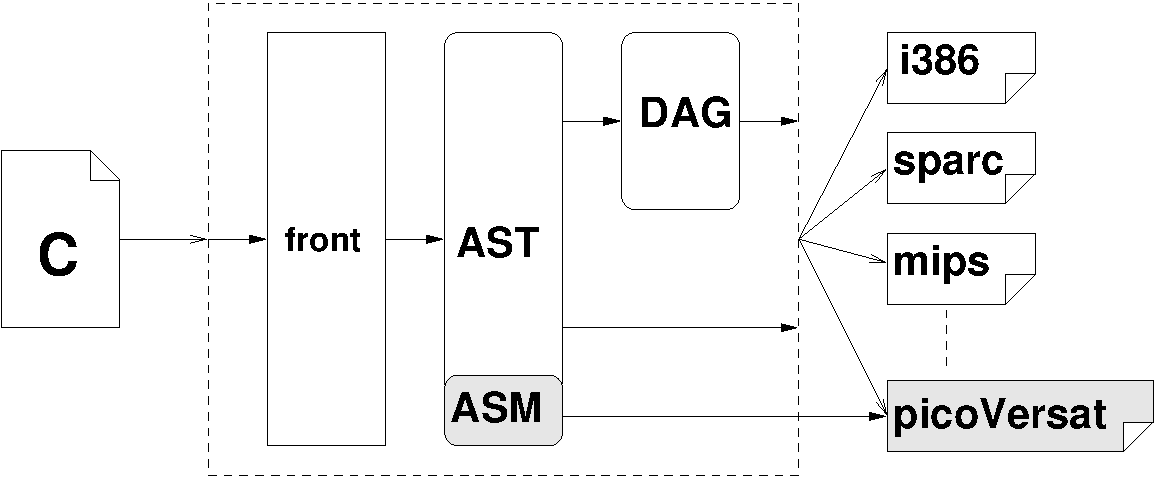
\includegraphics[width=0.9\textwidth]{Figures/lccPico.pdf}}
    \vspace{0cm}\caption{Changes in the {\bf lcc} blocks.}
    \label{fig:lccPico}
\end{figure}

\section{Data Engine Incorporation}

Even though {\it picoVersat} (Controller) can work on it's own for very simple
problems or auxiliary calculations, it's main purpose is to manage {\it Versat},
that is, all of its components.  In particular, the controller is meant to
manage the Data Engine in order to take full advantage of the accelerator.  This
is the biggest challenge when developing a compiler for this type of
architectures.

The code used to incorporate {\it Versat} support to the compiler needs to be
compatible with the code used to compile {\it picoVersat}.  Also, in an ideal
scenario, the compiler should not need to be different for compiling code with
or without the accelerator's functions, since the controller can operate
separately.
%This however might not be possible depending on the changes that might need to be made.

In order to make the control code for the {\it Versat} data engine compatible
with a {\bf C} language specification, instructions like {\tt
  alu0.connectPortA(aluLite0)} must be converted into {\tt connectPortA(alu, 0,
  aluLite, 0)}.  The later notation can then be parsed by any {\bf C} language
compatible preprocessor.
These instructions can be implemented as simple function call, for instance:
\begin{verbatim}
#define ALU_CONF_SELB_OFFSET 1
#define connectPortA(int a, in_a, int b, in_b) {
    asm("ldi %d\n", b[in_b]);
    asm("wrc %d, %d\n", a[in_a], ALU_CONF_SELB_OFFSET);
}
\end{verbatim}

%On the other hand, taking into account the required {\tt asm} support, they can
%be implemented as {\tt cpp} {\bf C} preprocessor macros, for instance:
%\begin{verbatim}
%#define connectPortA(a,b) \
%    asm("ldi s" #a "\n\twrc " #b "ALU_CONFIG_ADDR,ALU_CONF_SELA_OFFSET\n")
%\end{verbatim}

%trocar esta funcao para ver como um vetor e um indice como esta na de cima

The top level {\it Versat} loop can then be invoked through a {\tt versat()}
function that drives the above configuration specific routines.  This approach
replaces the complex {\tt for} instruction of the previous compiler, where some
values, as well as the inner structure, must have a specific format instead of
general purpose {\bf C} language {\tt for} instruction.  The routine parameters
correspond to the configuration parameters that define the operations to be
performed in each {\sc ALU}, the port connections, the cycle start value, delay,
period, {\em etc.}  Since there are a large number of parameters to be
specified, auxiliary structures can be used to group related information.  These
structures can then be used to determine differences from the previous
configuration uploaded to {\it Versat}, simplifying the partial configuration
task.

The {\tt versat()} function uses the parameters to determine the next
configuration to be made.
After checking the differences between the configuration currently stored in
the Configuration Module and the one calculated, a final configuration is determined.
This final configuration is made so that only the FUs that need to change their
functionality are incrementally updated, decreasing reconfiguration time
(partial reconfiguration).

The representation of the {\tt versat()} function has all of the
parameters necessary to get a new configuration as arguments.
For the current compiler, these parameters are extracted by analyzing a specific
{\tt for()} loop model, for instance:
\begin{verbatim}
for(j=0;j<R6;j++) {
    for(i=0;i<R14;i++) {
        mem0B[R1+j*R13+i] = (mem1A[R1+j*R13+i] * mem2B[1025+j*R2+R10*i]) -
                            (mem0A[R1+j*R13+i] * mem2A[1024+j*R2+R10*i]);
    }
}
\end{verbatim}

From this code block all the information needed in order to create a new data engine
configuration is present.
Therefor, the new formulation of these operations to be done in {\it Versat} must also
have the same core information.
For this purpose the function declaration is given by:
\begin{verbatim}
extern void versat(int N, int M, int* op, int* a, int* b, int* c, int* mem);
\end{verbatim}

This is possible since the operations to be done in the loops can be described by
a generic formula or combinations of it, for instance:
\begin{verbatim}
memory_x[a_x*i + b_x*j + c_x] = memory_y[a_y*i + b_y*j + c_y] operation
                                memory_z[a_z*i + b_z*j + c_z];
\end{verbatim}

As a result, by having {\tt a}, {\tt b}, {\tt c}, {\tt op} and {\tt mem} as vectors of
parameters that complete the formulation of these loop operations, the {\tt versat()}
function can be invoked with the necessary specifications, for instance:
\begin{verbatim}
#include "versat.h"
int main() {
    int *a, *b, *c, *op, *mem;
    int N, M;
    /* ... */
    /* insert values into parameters to get desired operations */
    versat(N, M, a, b, c, op, mem);
    /* ... */
    return 0;
}
\end{verbatim}

Alternatively, the structure containing all parameters, defined in
{\tt versat.h}, can be used to assign only the desired parameters,
or all of the parameters in sequence.
\begin{verbatim}
#define VERSAT_MEM0A 5120
#define VERSAT_FU 6176

typedef struct versatFU {
    struct mem { int iter, per, duty, sela, start, shift, incr, delay, rvrs; }
        mem0A, mem0B, mem1A, mem1B, mem2A, mem2B, mem3A, mem3B;
    struct alu { int sela, selb, fns; }
        alu0, alu1, alulite0, alulite1, alulite2, alulite3;
    struct mult { int sela, selb, lonhi, div2; }
        mult0, mult1, mult2, mult3;
    struct bs { int sela, selb, lna, lnr; } bs;
} Versat;

typedef struct versatDE {
    int mem0A, mem0B, mem1A, mem1B, mem2A, mem2B, mem3A, mem3B;
    int alu0, alu1, alulite0, alulite1, alulite2, alulite3;
    int mult0, mult1, mult2, mult3, bs0;
} VersatDE;
\end{verbatim}

Now, by including {\tt versat.h}, all parameters are accessible through
a single memory mapped structure initialized to the base address of each
parameter base.

\begin{verbatim}
#include "versat.h"
static int base = VERSAT_MEM0A, versatFU = VERSAT_FU;
int main() {
    Versat *versatFu = (Versat*)base;
    VersatDE *versatDE = (VersatDE*)versatFU;
    /* ... */
    return 0;
}
\end{verbatim}

Also, a structure can be defined with all required parameters and then copied
into the required memory position simply by {\bf C} structure assignment.

\begin{verbatim}
#include "versat.h"
static int base = VERSAT_MEM0A;
Versat config1 = { { 2000, 1, 1, 0, 0, 1, 1, 0, 0, } /* ... */ };
int main() {
    Versat *versatFu = (Versat*)base;
    /* ... */
    *versatFu = config1;
    /* ... */
    return 0;
}
\end{verbatim}


%For example creating a {\it MACRO} for the functions to be done in {\it Versat}, or creating sections that get separated by specific lines of code to identify the code portions that are meant to be done by the accelerator, or try do detect if a certain portion of code is in the correct for to be executed in {\it Versat} or even creating functions that operate with the accelerator that take as parameters what is needed to implement the configuration for each component.
